In this LIDAR lab oration the National instruments myRIO was used in combination with National instruments LabWIEV. 
When using myRIO as an base for the LIDAR there is a coupel of design considerations to take in to count especially if the LIDAR have the need to be fast because then the latency and the transfer speed of the USB can be a limitation. 
In this project it was decided to go with an spitted architecture letting the myRIO do the measurements and controlling the motor while the personal computer was used to display the data that the myRIO captured.

\subsection{The myRIO software}\label{subsection:myRIO}
\begin{figure}[ht]
    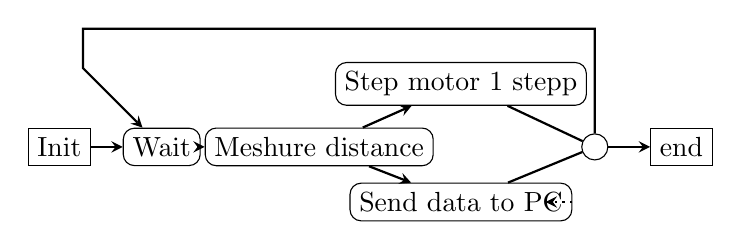
\begin{tikzpicture}
\tikzstyle{startstop} = [rectangle, rounded corners , minimum width=3mm, minimum height=1mm,text centered, draw=black]
\tikzstyle{round}=[circle, minimum width=0mm,draw=black]
\tikzstyle{first} = [rectangle, minimum width=1mm, draw=black]
\tikzstyle{empty}=[]

\usetikzlibrary{shapes.geometric, arrows}
\tikzstyle{arrow} = [thick,->,>=stealth]
\tikzstyle{dottarrow} = [thick, dotted,->,>=stealth]
\tikzstyle{noarrow}=[thick,-=,=stealth]

%nodes
\node (init) [first] {Init};
\node (wait) [startstop, right of =init, xshift=3mm] {Wait};
\node (mesh) [startstop, right of=wait, xshift=10mm] {Meshure distance};
\node (step) [startstop, right of=mesh, xshift=8mm ,yshift=8mm] {Step motor 1 stepp};
\node (send) [startstop, below of=step, yshift=-5mm]{Send data to PC};
\node (merge) [round, right of=mesh, yshift=0mm, xshift=25mm]{};
\node (end) [first, right of=merge, xshift=1mm] {end};
\node (topc) [empty, right of=send, xshift=2mm]{};

%arrows
\draw [arrow] (wait) -- (mesh);
\draw [arrow] (init) -- (wait);
\draw [arrow] (mesh) -- (step);
\draw [arrow] (mesh) -- (send);
\draw [noarrow] (send) -- (merge);
\draw [noarrow] (step) -- (merge);
\draw [dottarrow] (send) -- (topc);
\draw [arrow] (merge)  -- +(0,1.5)  -- (0.3,1.5) -- (0.3,1) -- (wait);
\draw [arrow] (merge) -- (end);
\end{tikzpicture}
  \caption{This figure describes the inner simplified working of the myRIO code.
  At the initiualising of the unit. Then because how the myRIO is working the code is waiting while the myRIO is measuring the sensor. The measure block only represents that we retrieve the value of the previously measured data. The data is put on the FIFO stack to b sent to the computer while myRIO takes an other step with the stepper motor. When that is done and the user haven't pressed stop to abort we loop back to wait and do the measurement again.}
  \label{fig:myRIO-loop}
\end{figure}
The myRIO part of the code uses an loop described in figure \ref{fig:myRIO-loop}.

\subsubsection{Measuring data}\label{subsubsection:mesure}
To decrease the shaking of the sensor the system ether needs to stop completely or not stop at all before measuring the distance.
Then the distance is acquired by using an analogue to digital converter.
After the distance have bin acquired the system stores the value as $y$ with the motor position $x$ in to a cluster and then in to an array of clusters. In this case the motor mentioned in \ref{section:hardware} have 400 steps and therefor the size of that array is 400 elements.

\subsubsection{Sending data to pc}\label{subsubsection:sendData}
The array previously mentioned in the section \ref{subsubsection:mesure} is sent over an network based shared variable that is implemented as an first in first out queue\cite{myRIO-Shared}.


\subsubsection{Step motor control}\label{subsubsection:Step-control}
Step motor control is achieved by using a implementation of a shift register explained in figure \ref{fig:shift-reg}. 

\begin{figure}[ht]
  \centering
  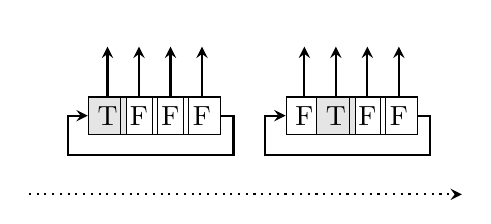
\begin{tikzpicture}
\tikzstyle{notused} = [rectangle, rounded corners , minimum width=3mm, minimum height=1mm,text centered, draw=black]
\tikzstyle{round}=[circle, minimum width=0mm,draw=black]
\tikzstyle{square} = [rectangle, minimum width=1mm, draw=black]
\tikzstyle{qraysquare} = [
rectangle, minimum width=1mm, draw=black, fill=gray!20]
\tikzstyle{empty}=[]

\usetikzlibrary{shapes.geometric, arrows}
\tikzstyle{arrow} = [thick,->,>=stealth]
\tikzstyle{dottarrow} = [thick, dotted,->,>=stealth]
\tikzstyle{noarrow}=[thick,-=,=stealth]

%node
\node (DA) [qraysquare] {T};
\node (DB) [square, right of =DA, xshift=-6mm] {F};
\node (DC) [square, right of =DB, xshift=-6mm] {F};
\node (DD) [square, right of =DC, xshift=-6mm] {F};

\node (DE) [square, right of =DD, xshift=3mm] {F};
\node (DF) [qraysquare, right of =DE, xshift=-6mm] {T};
\node (DG) [square, right of =DF, xshift=-6mm] {F};
\node (DH) [square, right of =DG, xshift=-6mm] {F};

%Epmty target nodes
\node (DAT) [empty, yshift=10mm]{};
\node (DBT) [empty, right of=DAT, xshift=-6mm]{};
\node (DCT) [empty, right of=DBT, xshift=-6mm]{};
\node (DDT) [empty, right of=DCT, xshift=-6mm]{};

\node (DET) [empty, right of=DDT, xshift=3mm]{};
\node (DFT) [empty, right of=DET, xshift=-6mm]{};
\node (DGT) [empty, right of=DFT, xshift=-6mm]{};
\node (DHT) [empty, right of=DGT, xshift=-6mm]{};

%lines to target node
\draw [arrow] (DA) -- (DAT);
\draw [arrow] (DB) -- (DBT);
\draw [arrow] (DC) -- (DCT);
\draw [arrow] (DD) -- (DDT);
\draw [arrow] (DD)  -- +(0.4,0) -- +(0.4,-0.5) -- (-0.5,-0.5) -+(-0.5,0.0) -- +(DA);

\draw [arrow] (DE) -- (DET);
\draw [arrow] (DF) -- (DFT);
\draw [arrow] (DG) -- (DGT);
\draw [arrow] (DH) -- (DHT);
\draw [arrow] (DH)  -- +(0.4,0) -- +(0.4,-0.5) -- (2.0,-0.5) -+(2.0,0.0) -- +(DE);

\draw [dottarrow] (-1.0cm,-1.0cm) -- (4.5cm,-1cm);

%node (D1) [square right of=Dfirst, xshift=8mm] {F};
%\node (D2) [square right of=D1, xshift=8mm] {F};
\end{tikzpicture}
  \caption{The shift register is working by step wise shifting the true state on step to the right and in this case have output upward. In this case the register is in state 1 at the left and proceed in the direction of the dotted arrow when moving over to the next state. When the true state reaches the right most cell it will on the next step be shifted to the beginning of the register. The output of this register is a 4 bit pararell bus denoted by the up facing arrows.}
  \label{fig:shift-reg}
\end{figure}
The motor is then pair wise connected to the each bit in the shift register thus implementing wave drive.

\subsection{Computer side}\label{subsection:computer-side}
The computer receives the data from the myRIO device and renders the result on the screen. In the figure \ref{fig:data-recive} a demonstration of the proces can be shown.

\begin{figure}[ht]
    \centering
   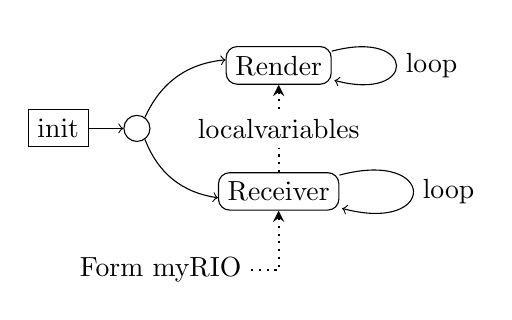
\begin{tikzpicture}
\tikzstyle{rounded} = [rectangle, rounded corners , minimum width=3mm, minimum height=1mm,text centered, draw=black]
\tikzstyle{round}=[circle, minimum width=0mm,draw=black]
\tikzstyle{square} = [rectangle, minimum width=1mm, draw=black]
\tikzstyle{empty}=[]

\usetikzlibrary{shapes.geometric, arrows}
\tikzstyle{arrow} = [thick,->,>=stealth]
\tikzstyle{dottarrow} = [thick, dotted,->,>=stealth]
\tikzstyle{dottline} = [thick, dotted,-,>=stealth]
\tikzstyle{noarrow}=[thick,-=,=stealth]

%nodes
\node (init) [square] {init};
\node (loop) [round, right of=init]{};
\node (render)[rounded, right of=loop, xshift=8mm, yshift=8mm ] {Render};
\node (rezive) [rounded, right of=loop, xshift=8mm, yshift=-8mm] {Receiver};
\node (datain) [empty, below of=rezive, xshift=-15mm]{Form myRIO};
\node (shared) [empty, below of=render, yshift=2mm]{localvariables};


%lines
%(Startnode)  edge [bend arrow]       node[text pos]  {text}          (target);
\path[->] 
(init) 		edge 								node[left]		{}			(loop)
(loop)		edge[bend left] 					node[left]		{}			(render)
(loop)		edge[bend right]					node[left]		{}			(rezive)
(render) 	edge[loop right]					node[right]		{loop}			(render)
(rezive) 	edge[loop right]					node[right]		{loop}			(rezive)
;
\draw [dottarrow] (datain) -| (rezive);
%\draw [dottarrow] (rezive) -- (render);
\draw [dottline] (rezive) -- (shared);
\draw [dottarrow] (shared) -- (render);

\end{tikzpicture}
  \caption{When the computer is runs the code. It first goes throw an initialisation phase that sets some common variables. After that it splits in 2 threads for with one is responsible for collecting the data from the myRIO and the other thread have the responsibility of rendering the user interface and the different graphical element.}
  \label{fig:data-recive}
\end{figure}

\subsubsection{Collecting the data form myRIO}\label{subsubsection:collectData}
Sins the myRIO sends the data in an array of clusters the program needs to extract the data in each $y$ value and convert the value that is based on voltage to an value that is based on distance. That conversion is done doing an exponential regression over value and range, more info about the regression can be found in chapter \ref{secition:results}. The compute then stores the cluster array in memory so it can be sent over to the other loop by using local variables.

\subsubsection{Rendering the Polar-plot}\label{subsubsection:renderPolar}
Rendering the polar plot is then done by sending that array in to the polar plot with point iteration\cite{labVIEW-polar-plot} in the render thread.
This is done because then render can run in a slower phase then the receiver and thus save decrees the power usage of the program.
As an side effect of this the screen is much more stable and don't blink as much.

\subsubsection{Computing the histogram}\label{subsubsection:comphistogram}
This program have a ability to generate a histogram view of the length based users inputted expected value defined as $\mu:=$"User expected value" and delta value $\Delta:=$"Users expected min/max" that is going to be used to calculated an expected min and max value defined as $ max:=\mu+\Delta,\quad min:=\mu-\Delta, \quad D:=$"Distance to object".
The computation is done by first taking each measurement and checking if the value of the data is in the interval of $ (min \leq D \leq max) $ then if so restore the data as an frequency array by using the distance as indexer in the array and increasing the value in that cell by one.
Value that occurs outside the expected min/max interval is ignored.
In this way the histogram plot even works for detecting mean and standard deviation while rotating in an \textbf{lees} deterministic environment.
After rotating by any number of turns the software can calculate the mean and standard deviation using the formulas down below.
$$\begin{matrix} 
\overline{x}=\frac{\Sigma(x_i-\mu)^2}{\Sigma(y_i)} & 
\sigma= \sqrt{\frac{\Sigma((f_i*x_i-\overline{x})^2)}{\Sigma(f_i)}}
\end{matrix}\label{equation:mean-and-div}$$
The figure is rendered using labVIEWs "plot waveform vi" \cite{labVIEW-Plot-Waveform-VI}.
